\documentclass[11pt,a4paper]{article}

% ----------------- Pacotes básicos -----------------
\usepackage[utf8]{inputenc}
\usepackage[T1]{fontenc}
\usepackage[brazil]{babel}
\usepackage{lmodern}
\usepackage{geometry}
\geometry{margin=2.5cm}
\usepackage{setspace}
\onehalfspacing

% ----------------- Matemática e figuras -----------------
\usepackage{amsmath, amssymb, amsfonts}
\usepackage{siunitx}
\usepackage{graphicx}
\usepackage{booktabs}
\usepackage{float}

% ----------------- Código (listings) -----------------
\usepackage{listings}
\usepackage{xcolor}
\lstdefinestyle{mystyle}{
  basicstyle=\ttfamily\small,
  keywordstyle=\color{blue!60!black}\bfseries,
  commentstyle=\color{green!40!black}\itshape,
  stringstyle=\color{orange!60!black},
  numbers=left,
  numberstyle=\tiny\color{gray},
  stepnumber=1,
  numbersep=8pt,
  breaklines=true,
  frame=single,
  framerule=0.3pt,
  tabsize=2,
  showstringspaces=false
}
\lstset{style=mystyle, language=Python}

% ----------------- Hiperlinks -----------------
\usepackage[hidelinks]{hyperref}

\title{Pipeline de Indicadores Macroeconômicos e Modelos de Séries Temporais (VAR, VECM, PCA--ARX e Markov-Switching)}
\author{Relatório Técnico}
\date{\today}

\begin{document}
\maketitle
\tableofcontents
\newpage

\section{Visão geral}
Este relatório documenta:
\begin{itemize}
    \item O \textbf{pipeline de coleta e preparação} de dados macroeconômicos (últimos 10 anos), que produz um Excel consolidado em:
    \[
      \texttt{C:\textbackslash Users\textbackslash Lenovo\textbackslash Desktop\textbackslash Desktop\textbackslash Mestrado FGV\textbackslash IndicadoresMacro\textbackslash indicadores\_macro.xlsx}
    \]
    \item Quatro \textbf{modelos de séries temporais} aplicados aos dados salvos:
    \begin{enumerate}
        \item VAR (previsão multivariada e IRFs);
        \item VECM (cointegração em níveis, ex.: câmbio e diferencial de juros);
        \item PCA--ARX (fatores dinâmicos para prever retorno do Ibovespa);
        \item Markov-Switching (mudança de regime de volatilidade/retornos).
    \end{enumerate}
\end{itemize}

\section{Atualizações do pipeline (versão atual)}
\begin{itemize}
  \item \textbf{Treasury 10 anos (\% a.a.)}: inclusão de \emph{fix} automático de \emph{unidade}. Se a mediana vier em fração (e.g., 0{,}04 = 4\%), o script multiplica por 100; se vier \(\approx 0{,}4\) (deveria ser 4{,}0), multiplica por 10. Fallback permanece \texttt{\^{}TNX}/10.
  \item \textbf{PIB EUA (\% a/a)}: passa a ser baixado do FRED (\texttt{A191RL1Q225SBEA}), marcado no fim do trimestre e reamostrado para ME.
  \item \textbf{Crédito/Endividamento/Inadimplência}: mapeamento ampliado (PF, PJ, livres, total, \%PIB e \% renda).
  \item \textbf{Estrutura para Ipeadata/SIDRA/SGS extra}: dicionários de mapeamento (\texttt{IPEA\_MAP}, \texttt{SIDRA\_MAP}, \texttt{SGS\_EXTRA}) prontos para ativar novas séries sem mudar o pipeline.
  \item \textbf{Metadados e médias anuais}: aba adicional com médias anuais (média simples das observações mensais de cada ano).
\end{itemize}

\section{Pipeline de dados (resumo do código)}
\subsection{Janela temporal e agregação}
A amostra cobre os \textbf{últimos 10 anos} até o \emph{último mês fechado}. Séries diárias são \textbf{reamostradas para ME} (\emph{month-end}) por \texttt{last} ou \texttt{mean}.

\subsection{Fontes e robustez}
\paragraph{Yahoo Finance} com \texttt{yfinance} (coluna \emph{Adj Close} ou \emph{Close}).
\paragraph{PTAX (Olinda/BCB)} com fatiamento anual e \textbf{fallback} para \texttt{USDBRL=X}.
\paragraph{SGS (python-bcb)} com janelas de 5 anos e concatenação.
\paragraph{FRED} (DGS10, DFEDTARU/DFEDTARL, PIB EUA YoY). Fallback UST10 por \texttt{\^{}TNX}/10 quando necessário.

\section{Transformações para modelagem}
\begin{itemize}
  \item Índices/preços: \(\Delta \ln x_t\) (retornos/crescimentos);
  \item Juros: \texttt{pct\_change};
  \item VAR em estacionários; VECM para níveis \(I(1)\) quando houver cointegração.
\end{itemize}

\section{Resultados empíricos mais recentes}
Esta seção resume \textbf{os resultados que você rodou} com o Excel gerado pela versão atual do pipeline.

\subsection{VAR (6 variáveis, seleção por AIC)}
\paragraph{Especificação.} \(y_t = \{\Delta \ln \text{IBC}, \Delta \ln \text{USD/BRL}, \Delta \ln \text{Brent}, \Delta \ln \text{S\&P500}, \Delta \text{Selic}, \Delta \text{UST10}\}\).

\paragraph{Coeficientes relevantes (p-valores).}
\begin{itemize}
  \item \textbf{Atividade (}\(\Delta \ln \text{IBC}\)\textbf{)}: efeito negativo de \(\text{UST10}_{t-1}\) sobre o crescimento (p \(\approx 0{,}003\)).
  \item \textbf{Brent}: \(\text{ret\_spx}_{t-1}\) positivo (p \(\approx 0{,}044\)) e \(\text{UST10}_{t-1}\) positivo (p \(\approx 0{,}013\)).
  \item \textbf{S\&P 500}: inércia negativa em \(t-4\) (p \(\approx 0{,}029\)); \(\text{Selic}_{t-5}\) positiva (p \(\approx 0{,}009\)); \(\Delta \ln \text{Brent}_{t-8}\) negativa (p \(\approx 0{,}012\)); \(\text{Selic}_{t-9}\) positiva (p \(\approx 0{,}045\)).
  \item \textbf{Selic}: \(\Delta \ln \text{IBC}_{t-2}\) positiva (p \(\approx 0{,}031\)); \(\text{ret\_spx}_{t-2}\) positiva (p \(\approx 0{,}004\)); \(\text{UST10}_{t-3}\) positiva (p \(\approx 0{,}036\)); \(\Delta \ln \text{USD/BRL}_{t-7}\) positiva (p \(\approx 0{,}029\)).
  \item \textbf{UST10}: persistência (\(\text{UST10}_{t-2}\), p \(\approx 0{,}025\)); ligações com Brent (\(+\) em \(t-6\), p \(\approx 0{,}014\); \(-\) em \(t-11\), p \(\approx 0{,}015\)); e com \(\text{ret\_spx}_{t-10}\) (p \(\approx 0{,}029\)).
\end{itemize}

\paragraph{IRFs.} As funções resposta ao impulso (Figura~\ref{fig:irf}) mostram impactos moderados e bandas largas; choques de \textbf{UST10} tendem a reduzir o crescimento do \textbf{IBC} nos meses seguintes; \textbf{Brent} e \textbf{S\&P} se influenciam mutuamente.

\begin{figure}[H]
  \centering
  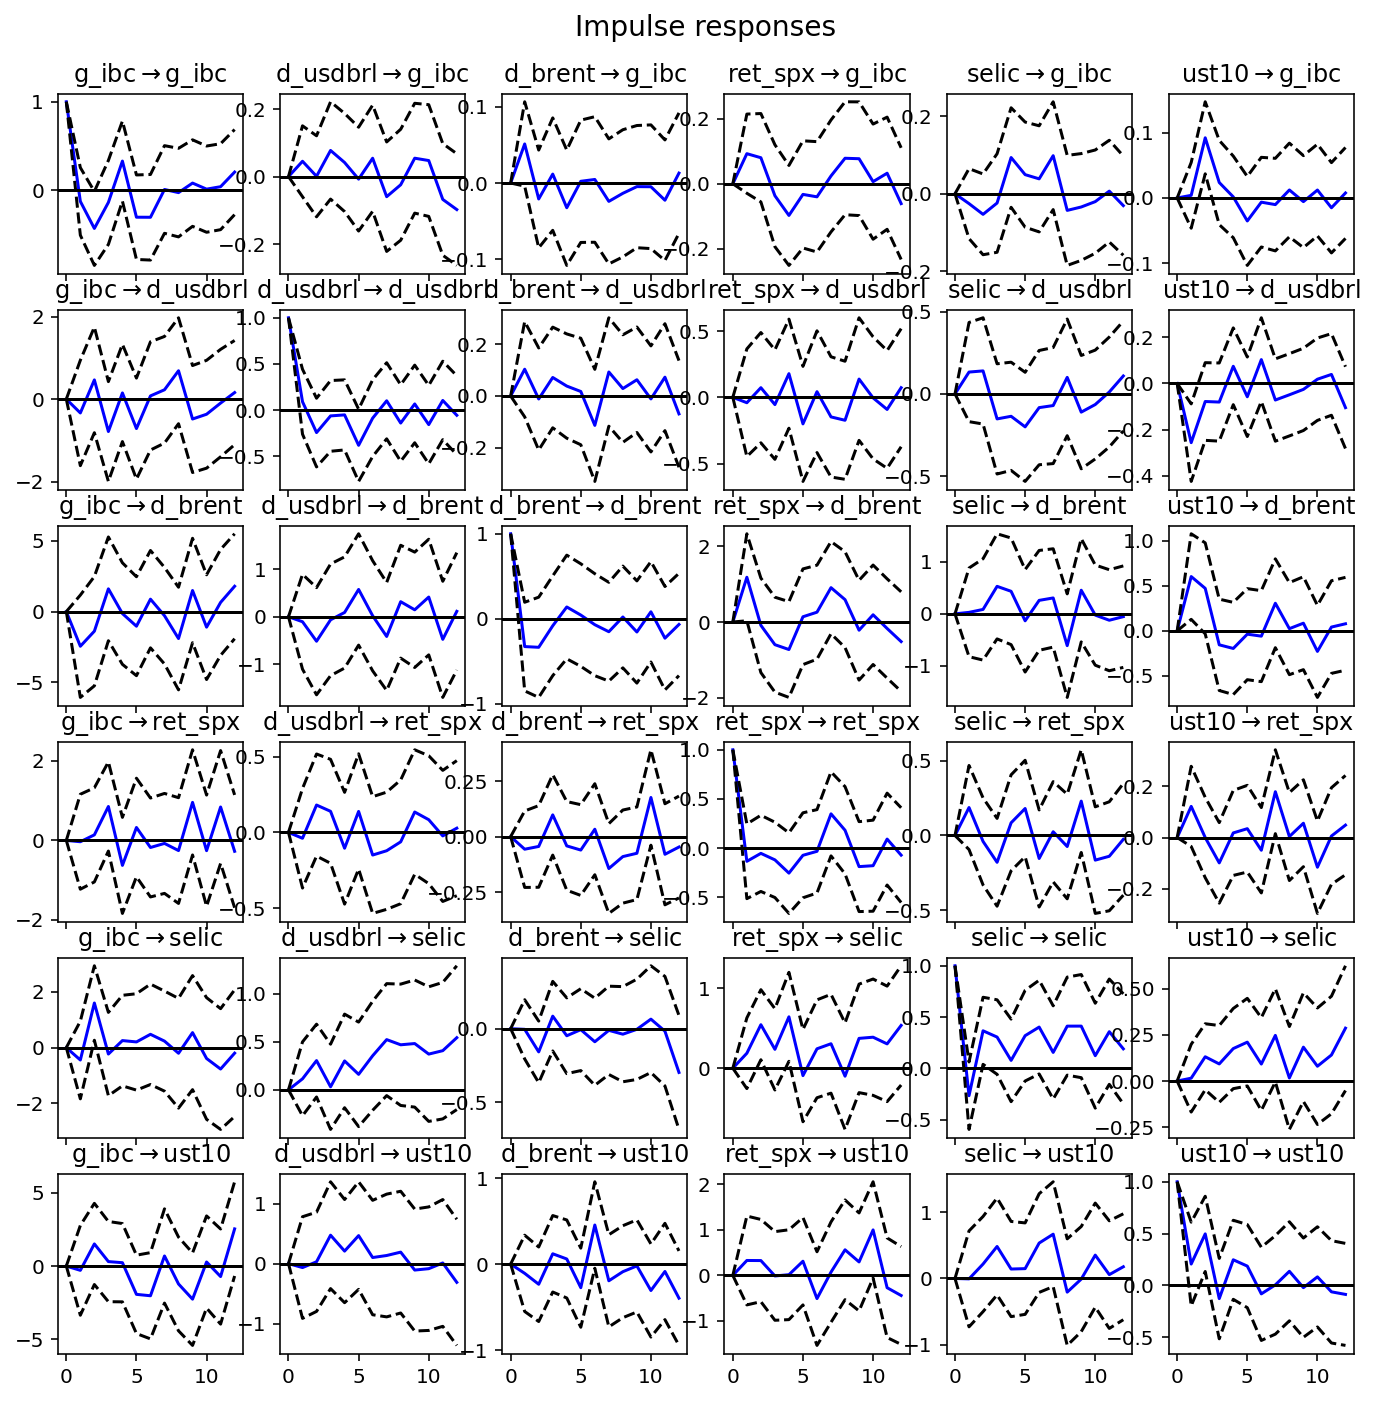
\includegraphics[width=\textwidth]{\detokenize{C:/Users/Lenovo/Desktop/Desktop/Mestrado FGV/IndicadoresMacro/Figure 2025-09-24 181629.png}}
  \caption{IRFs do VAR (horizonte de 12 meses).}
  \label{fig:irf}
\end{figure}

\paragraph{Previsão (12 meses).} As variações mensais previstas são pequenas (reversão à média). Primeiras 5 linhas (ilustrativo):
\begin{center}
\begin{tabular}{lrrrrrr}
\toprule
\textbf{Data} & $\Delta\ln$IBC & $\Delta\ln$USD & $\Delta\ln$Brent & $\Delta\ln$S\&P & $\Delta$Selic & $\Delta$UST10\\
\midrule
2025-08-31 & 0{,}027 & -0{,}028 & 0{,}033 & 0{,}024 & 0{,}021 & -0{,}076\\
2025-09-30 & -0{,}010 & 0{,}042 & -0{,}112 & 0{,}012 & 0{,}001 & 0{,}068\\
2025-10-31 & -0{,}015 & 0{,}014 & -0{,}025 & -0{,}030 & 0{,}055 & -0{,}176\\
2025-11-30 & -0{,}015 & 0{,}066 & -0{,}203 & -0{,}056 & 0{,}001 & -0{,}006\\
2025-12-31 & -0{,}008 & -0{,}002 & -0{,}032 & 0{,}036 & -0{,}027 & -0{,}079\\
\bottomrule
\end{tabular}
\end{center}

\subsection{VECM (USD/BRL e spread SELIC--Fed)}
\paragraph{Teste de Johansen.} Estatística traço \(= 13{,}38\) para \(r=0\) e críticos de 95\% \(=15{,}49\); para \(r=1\), traço \(=4{,}72\) e crítico \(=3{,}84\). \textbf{Conclusão}: não há cointegração a 95\% na amostra corrente (spread com \emph{proxy} UST10 em vez do Fed Funds real).
\paragraph{Implicação.} VECM não é indicado nesta configuração; use VAR em diferenças ou reestime com \textbf{Fed Funds} via FRED (média da banda) e/ou amostra mais longa.

\subsection{PCA--ARX (retorno do Ibovespa)}
\paragraph{Ajuste.} \(R^2 \approx 0{,}7\%\); coeficientes dos fatores não significativos; intercepto quase significativo (p \(\approx 0{,}052\)).
\paragraph{Sinal de 1 passo} (mês seguinte): \(\widehat{r}_{t+1} \approx \mathbf{0{,}009}\) (cerca de 0{,}9\%).
\paragraph{Leitura.} Em base mensal e usando apenas 2 fatores macro/mercado, o poder preditivo é baixo — condizente com literatura. Sugere-se testar horizontes mais longos, mais fatores e validação fora da amostra.

\subsection{Markov-Switching (2 regimes)}
\paragraph{Ajuste atual.} AIC \(-398{,}4\); porém, as probabilidades suavizadas colapsaram para \(\approx 1{,}0\) em sequência e houve \texttt{ConvergenceWarning} e matriz quase singular.
\paragraph{Diagnóstico.} \emph{Colapso de regime} (um regime com variância quase zero). Provável causa: escala dos dados ou especificação muito restrita.
\paragraph{Correções sugeridas.}
\begin{itemize}
  \item Usar \textbf{retornos padronizados} \((r-\bar r)/\sigma\);
  \item Estimar com \texttt{switching\_mean=True} além de \texttt{switching\_variance=True};
  \item Fornecer chutes/EM (\texttt{em\_iter=10}) e aumentar \texttt{maxiter};
  \item Se persistir, testar 3 regimes.
\end{itemize}

\section{Como executar}
\subsection*{Pré-requisitos de Python}
\begin{itemize}
  \item \texttt{pandas, numpy, requests, yfinance, statsmodels, scikit-learn, python-dateutil};
  \item FRED: definir \texttt{FRED\_API\_KEY} no ambiente (para Fed Funds \& PIB EUA);
  \item SGS: \texttt{python-bcb}.
\end{itemize}

\subsection*{Fluxo}
\begin{enumerate}
  \item Rodar o \textbf{pipeline} (\texttt{indicadores\_macro.xlsx});
  \item Rodar os blocos dos modelos (1 a 4).
\end{enumerate}

\section{Diagnósticos e cuidados}
\begin{itemize}
  \item Conferir \textbf{metadados} quando houver \emph{fallbacks};
  \item Em \texttt{pandas}, preferir frequência \textbf{ME} (aviso de depreciação para ``M'');
  \item VAR: verificar \emph{estabilidade} e autocorrelação dos resíduos; FEVD e Granger ajudam na interpretação;
  \item Estratégias: incorporar custos e gestão de risco.
\end{itemize}

\section{Extensões}
\begin{itemize}
  \item Ativar Ipeadata/SIDRA/SGS extra (IPCA, confiança, fiscal/dívida, desemprego);
  \item DFM/Kalman e TVP-VAR; combinação de sinais condicionada ao regime do Markov.
\end{itemize}

\end{document}